
\begin{figure}[H]
  {
    \setlength{\tabcolsep}{3.0pt}
    \setlength\cmidrulewidth{\heavyrulewidth} % Make cmidrule = 
    \begin{adjustbox}{height=5cm,center}
      \footnotesize
      \begin{tabular}{ll}

        \makecell[l]{
\icode{.BYTE \$00,\$01,\$01,\$01,\$00,\$FF,\$FF,\$FF}\\
\icode{.BYTE \$FF,\$FF,\$00,\$01,\$01,\$01,\$00,\$FF}
} & \makecell[l]{

\includegraphics[width=1.3cm]{src/patterns/pixels/pixel_pattern0_0.png}%
} \\
        \midrule

        \makecell[l]{
\icode{.BYTE \$00,\$02,\$00,\$FE}\\
\icode{.BYTE \$FE,\$00,\$02,\$00}
} & \makecell[l]{

\includegraphics[width=1.3cm]{src/patterns/pixels/pixel_pattern0_1.png}%

\includegraphics[width=1.3cm]{src/patterns/pixels/pixel_pattern0_2.png}%
} \\
        \midrule

        \makecell[l]{
\icode{.BYTE \$00,\$03,\$00,\$FD}\\
\icode{.BYTE \$FD,\$00,\$03,\$00}
} & \makecell[l]{

\includegraphics[width=1.3cm]{src/patterns/pixels/pixel_pattern0_3.png}%

\includegraphics[width=1.3cm]{src/patterns/pixels/pixel_pattern0_4.png}%

\includegraphics[width=1.3cm]{src/patterns/pixels/pixel_pattern0_5.png}%
} \\
        \midrule

        \makecell[l]{
\icode{.BYTE \$00,\$04,\$00,\$FC}\\
\icode{.BYTE \$FC,\$00,\$04,\$00}
} & \makecell[l]{

\includegraphics[width=1.3cm]{src/patterns/pixels/pixel_pattern0_6.png}%
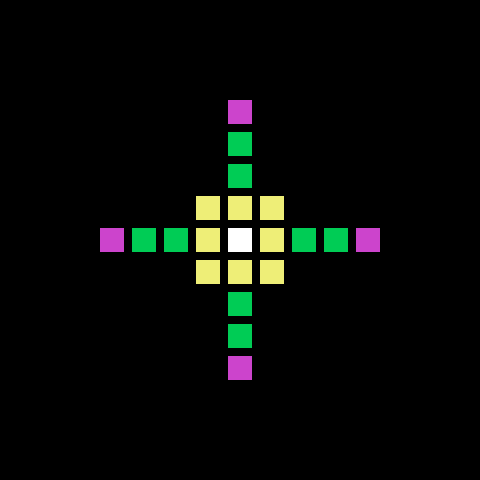
\includegraphics[width=1.3cm]{src/patterns/pixels/pixel_pattern0_7.png}%
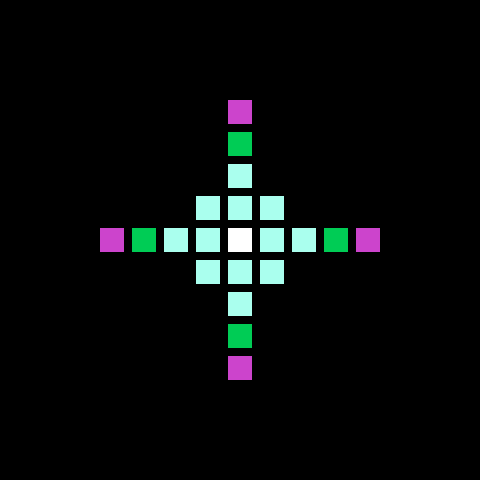
\includegraphics[width=1.3cm]{src/patterns/pixels/pixel_pattern0_8.png}%
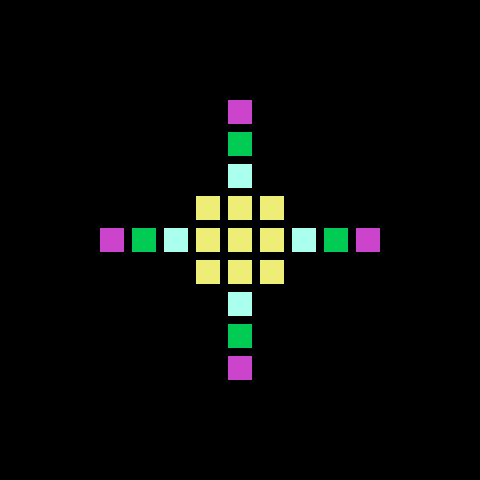
\includegraphics[width=1.3cm]{src/patterns/pixels/pixel_pattern0_9.png}%
} \\
        \midrule

        \makecell[l]{
\icode{.BYTE \$FF,\$01,\$05,\$05,\$01,\$FF,\$FB,\$FB}\\
\icode{.BYTE \$FB,\$FB,\$FF,\$01,\$05,\$05,\$01,\$FF}
} & \makecell[l]{
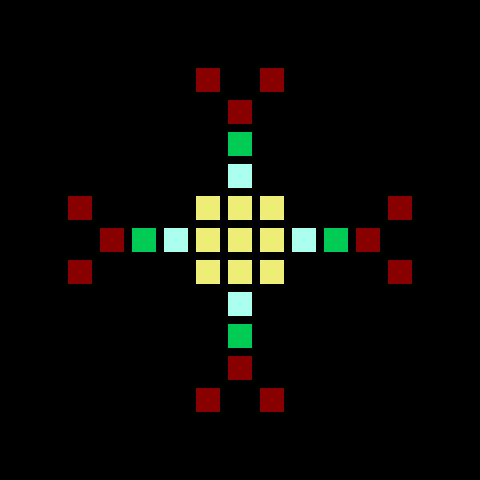
\includegraphics[width=1.3cm]{src/patterns/pixels/pixel_pattern0_10.png}%
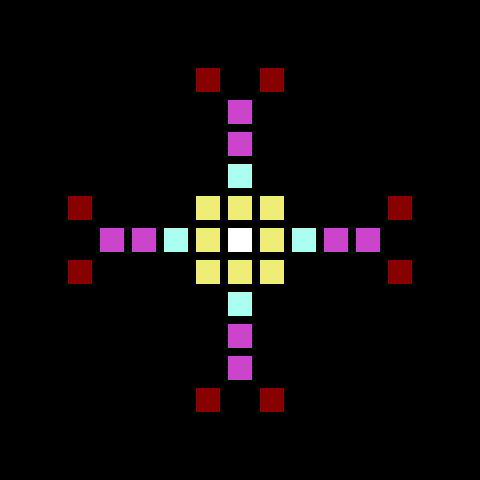
\includegraphics[width=1.3cm]{src/patterns/pixels/pixel_pattern0_11.png}%
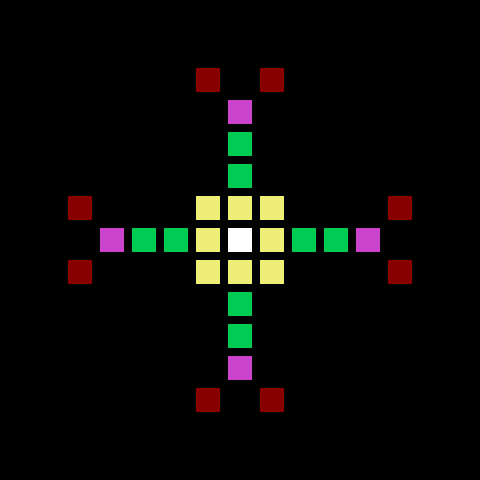
\includegraphics[width=1.3cm]{src/patterns/pixels/pixel_pattern0_12.png}%
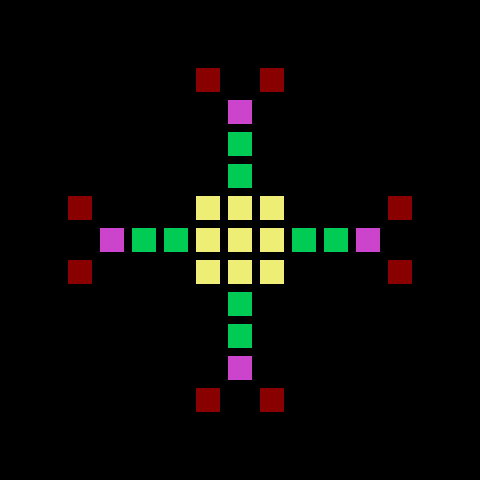
\includegraphics[width=1.3cm]{src/patterns/pixels/pixel_pattern0_13.png}%
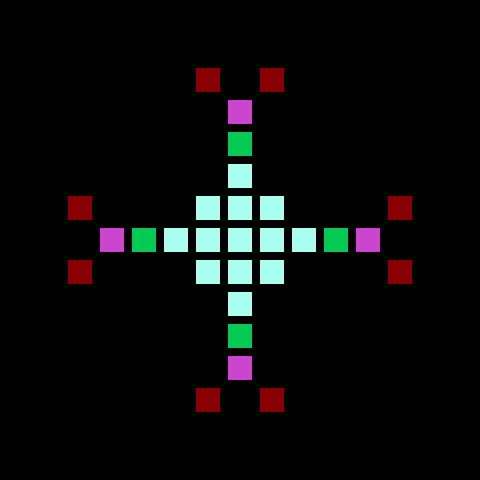
\includegraphics[width=1.3cm]{src/patterns/pixels/pixel_pattern0_14.png}%
} \\
        \midrule

        \makecell[l]{
\icode{.BYTE \$00,\$07,\$00,\$F9}\\
\icode{.BYTE \$F9,\$00,\$07,\$00}
} & \makecell[l]{
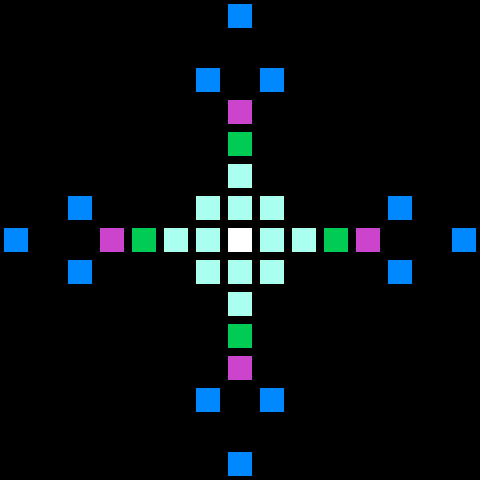
\includegraphics[width=1.3cm]{src/patterns/pixels/pixel_pattern0_15.png}%
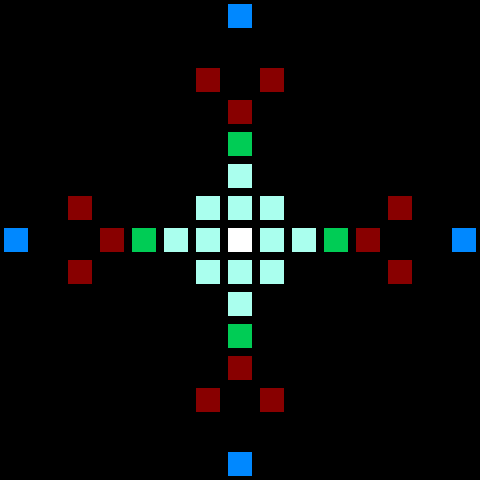
\includegraphics[width=1.3cm]{src/patterns/pixels/pixel_pattern0_16.png}%
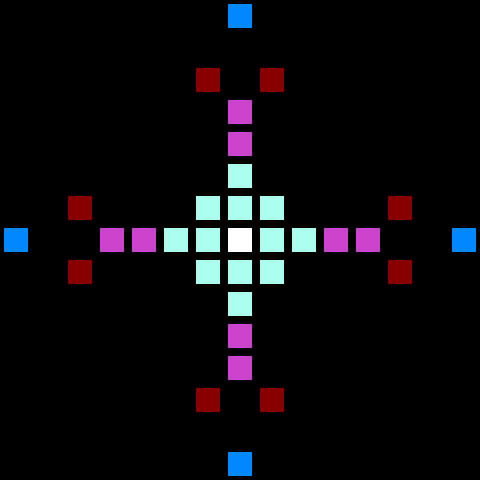
\includegraphics[width=1.3cm]{src/patterns/pixels/pixel_pattern0_17.png}%
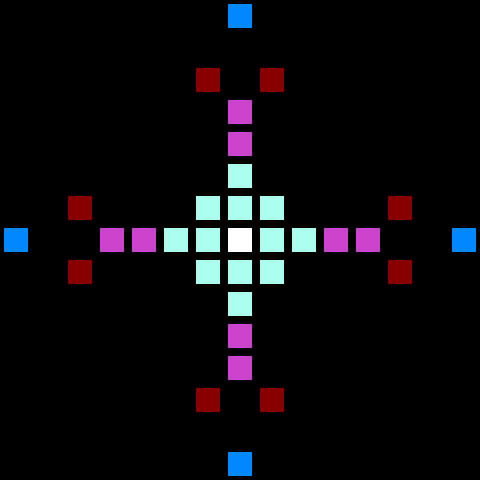
\includegraphics[width=1.3cm]{src/patterns/pixels/pixel_pattern0_18.png}%
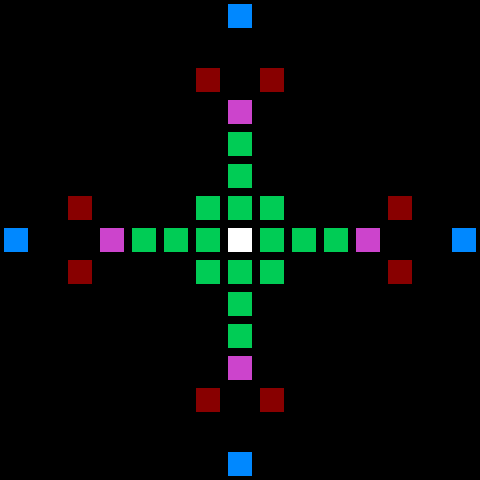
\includegraphics[width=1.3cm]{src/patterns/pixels/pixel_pattern0_19.png}%
} \\
        \midrule

        \makecell[l]{
\icode{.BYTE}\\
\icode{.BYTE}
} & \makecell[l]{
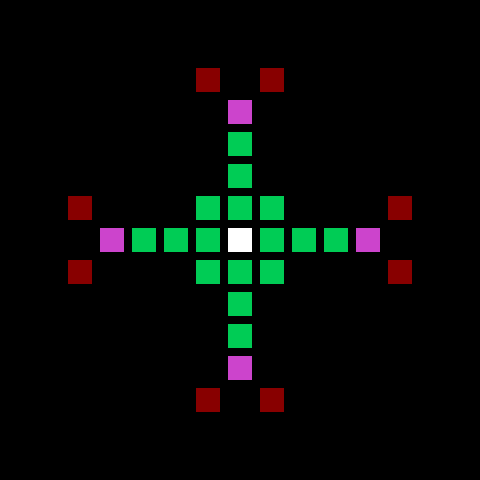
\includegraphics[width=1.3cm]{src/patterns/pixels/pixel_pattern0_20.png}%
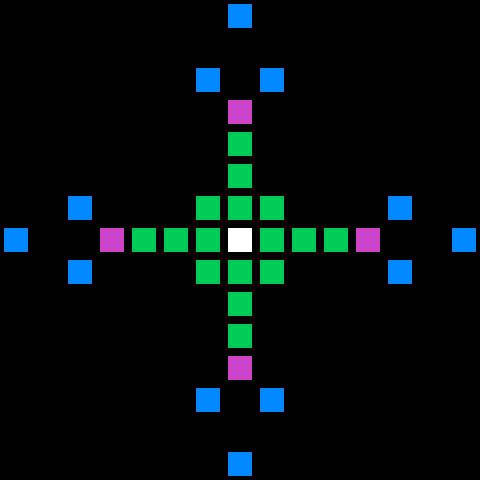
\includegraphics[width=1.3cm]{src/patterns/pixels/pixel_pattern0_21.png}%
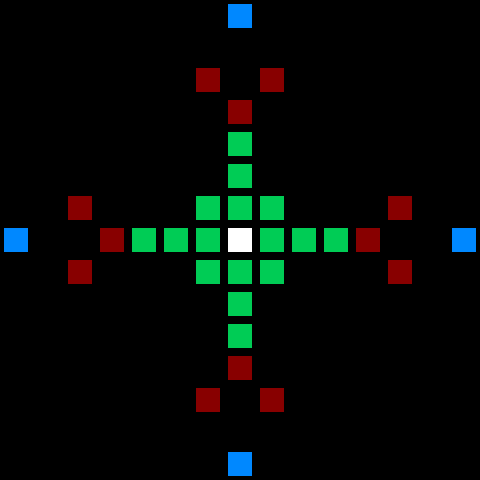
\includegraphics[width=1.3cm]{src/patterns/pixels/pixel_pattern0_22.png}%
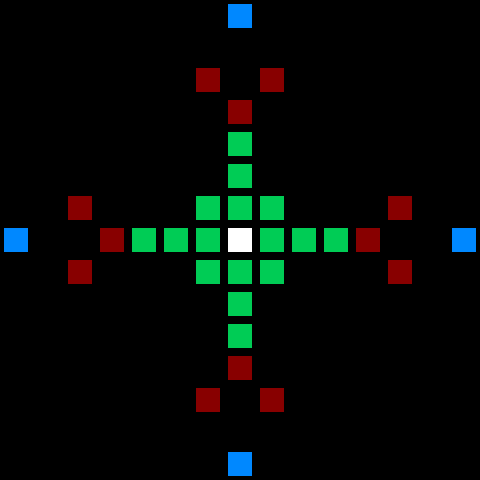
\includegraphics[width=1.3cm]{src/patterns/pixels/pixel_pattern0_23.png}%
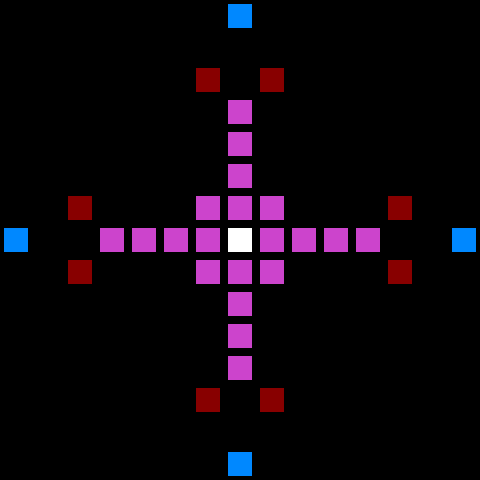
\includegraphics[width=1.3cm]{src/patterns/pixels/pixel_pattern0_24.png}%
} \\
        \midrule

      \end{tabular}
    \end{adjustbox}
  }\caption{The purpose of each of the oscillator values.}
\end{figure}
